% \par
% In this chapter, we will see and discuss the implementation of different proposed solutions for the document classification problem. We will discuss both the Convolutional Neural Networks, based on textual input and images, trained for the problem. As we mentioned in the previous chapter that we used transfer learning for one of our ConvNet model so we will also discuss the reason for choosing this methodology. Furthermore, based on these methodologies, we have carried out some experiments on our dataset, which we will also evaluate and compare different solutions. Along with that, we will briefly discuss the technology stack and evaluation metrics used in the solution. We broke the implementation chapter into different sections respective to the provided solution and will see each solution one by one.

In this section, we will discuss the methodology and implementation of solution for lane detection using CNN. We will also elaborate how we used a popular CNN architechure for our use case. Furthermore, we carried out some experiments on our dataset to know whether our choosen CNN architechure is able to detect lanes or not. Before that, we will briefly discuss the technologies and tools used for data gathering, implementation and evaluation metrics used in the solution. This chapter is divided into separate sections as mentioned above.

\section{Technology Stack}
\subsection{Unity3D}\label{subsec:unity}
Unity3D is a powerful cross-platform game engine with user-friendly development APIs and environment and is developed by Unity Technologies. It is very easy to begin with and is flexible enough for the expert game developers. Unity is oftenly used to easily create 3D games and applications for mobile, desktop, the web, and consoles. Simulating real-world has saved researchers and scientists has not only provided safe environment but also saved millions of dollars in testing their proposed solutions. Unity3D is also being used in developing interactive simulations and visualizations. Using a real-time 3D virtual world simulated in Unity3d, you can re-enact and test multiple complex scenarios, and understand how you products will perform without putting significant investment in hardware.

\par
Unity3D\cite{unity3d} provides off-the-shelf content to enhance you project and make development easier, organized and faster. These multiple Standard Assets include: Cameras, Characters, Effects, Environment, ParticleSystems, Utility, Prototyping, Vehicles, CrossPlatformInput. Unity’s Asset Store is a library containing free and paid assets created both by Unity Technologies and also members of the Unity community. A lot of variety of assets is available for example models, animations, textures, editor extensions, tutorials or even whole projects.

\subsection{EasyRoads3D}\label{subsec:easyroad3d}
EasyRoads3D\cite{easyroads3d} is a toolset can be imported from Unity's Asset Store and is used to create other infrastructures such as unique road networks and rivers with the riverbed carved in the terrain, using Unity3D. It is a paid asset. You can use fully customizable built-in system of EasyRoads3D or import our own assets to create different road networks from scenic environments to complex urban road networks. It comes with an extremely useful tool of side objects. The side objects tool allows the creation of individual objects like walls, fences, houses, plant vegetation, etc.

\begin{figure}[H]
  \centering
  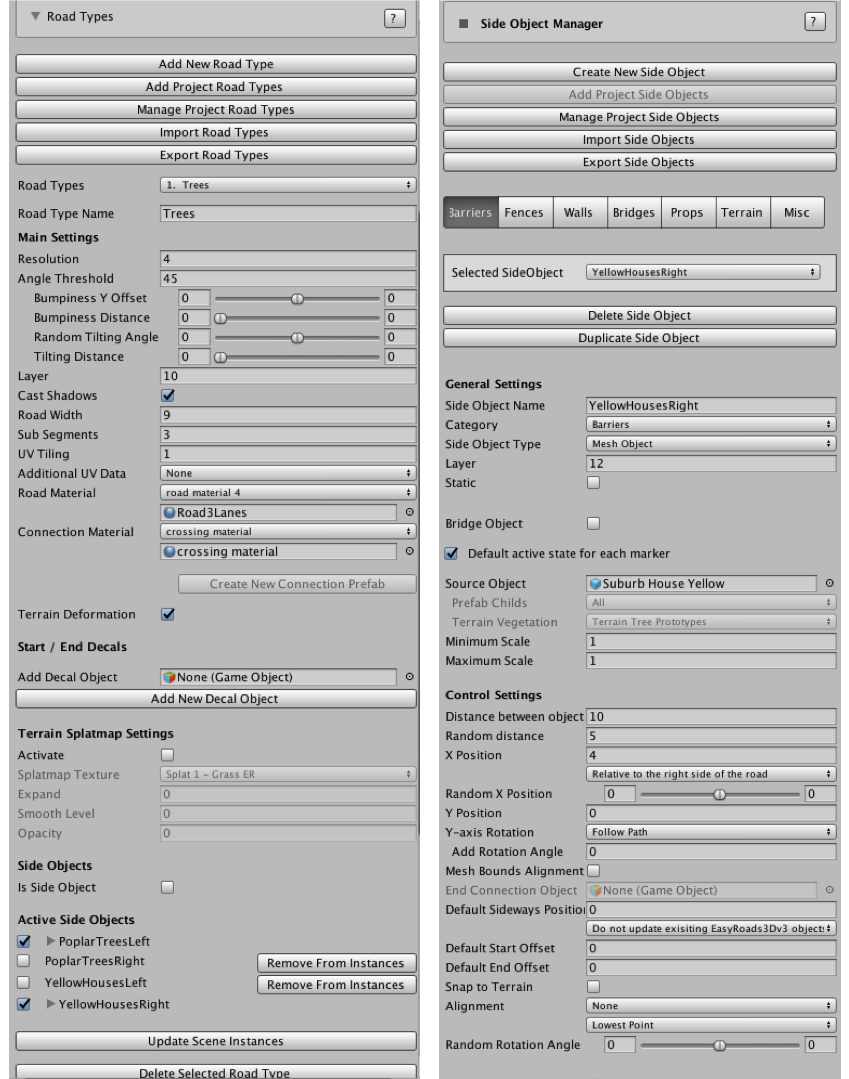
\includegraphics[scale=0.50]{images/Chapter4/easyroad3d.png}
  \caption{EasyRoad3D Unity Inspector}
  \label{fig:remote_ssh}
\end{figure}

\subsection{VSCode}
Visual Studio Code (VSCode)\cite{vscode} is a cross-platform source-code editor developed by Microsoft. It blends the ease of a source code editor with powerful developer tools such as debugging, IntelliSense code completion and integrated terminal. The edit-build-debug cycle is smooth and effortless which means more time to work on your ideas and rather than fiddling with your environment. VSCode is very customizable and extensible by installing extensions to add more features. Some of the notable extensions that I have installed for this project are:
\begin{itemize}
  \item \textbf{Python Extension:} VSCode ships with Javascript, TypeScript, CSS, and HTML language support. Since we are using Python language for training our machine learning model, we can add Python \ref{subsec:python} language support by installing Python plugin\cite{vscode_python}. It not only supports code completion and IntelliSense. IntelliSense is a general term for a number of features, including intelligent code completion (in-context method and variable suggestions) across all your files and for third-party and built-in modules. It shows you methods, class members, and documentation as you type, and allows you to trigger completions at any time. This plugin also allows you to set breakpoints on Python code, inspect data, and use the debug console as you run your program step by step. It also add supports linting of your Python code for potential errors, making it easy to jump to particular section of code and correct different problems.

  \item \textbf{Remote: SSH} 
  The Remote - SSH extension\cite{vscode_remote_ssh} allows you to use and open files and folders hosted on any remote machine with a SSH server as your development environment and take full advantage of VSCode's features. This can help streamline development and troubleshooting in a wide variety of scenarios. For example, you can develop use larger, faster, or more specialized hardware than your local machine or directly develop on deployment machine. Moving between various remote development environments and making changes safely without thinking about the effects of your local machine becomes easy. You can also troubleshoot a program that is deployed anywhere else, such as a customer site or in the cloud.
  \par
  \begin{figure}[H]
    \centering
    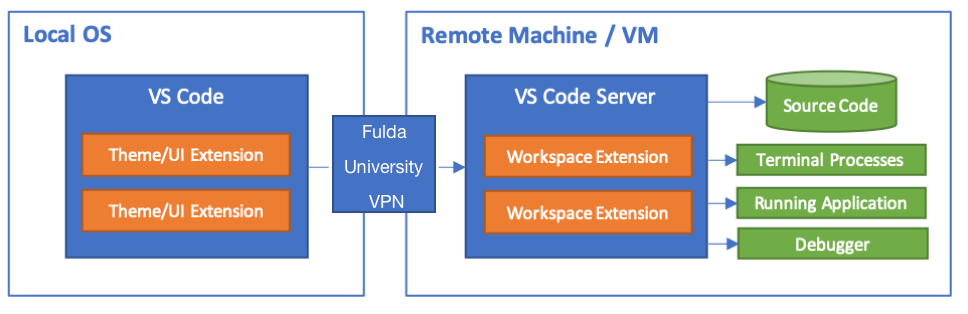
\includegraphics[scale=0.80]{images/Chapter4/architecture-ssh.png}
    \caption{VSCode - Remote SSH plugin Architecture}
    \label{fig:remote_ssh}
  \end{figure}
  In our case, we are using a GPU-heavy cluster machine in Hochschule Fulda for training our machine learning model as my machine has not much resources to train our model with such a large dataset. We could have used Gedit\cite{gedit} or Vim\cite{vim} but it would not have rich features of VSCode. We can only access the cluster through connecting to Hochschule Fulda's VPN. So we set up a simple SSH Tunnel to the cluster through the VPN. We used a \q{configuration file}\cite{config_file} to store the connection as shown in Figure \ref{fig:ssh_connection}, which is supported by OpenSSH, to store all your different SSH connections. Then, we setup \q{key based authentication}\cite{key_based_auth} to login without entering password. Then we can easily use the Remote SSH extension to connect to the cluster. leverage all of the great features of VS Code such as IntelliSense (completions), code navigation, and debugging, as if we were working locally.
  \begin{figure}[H]
      \centering
      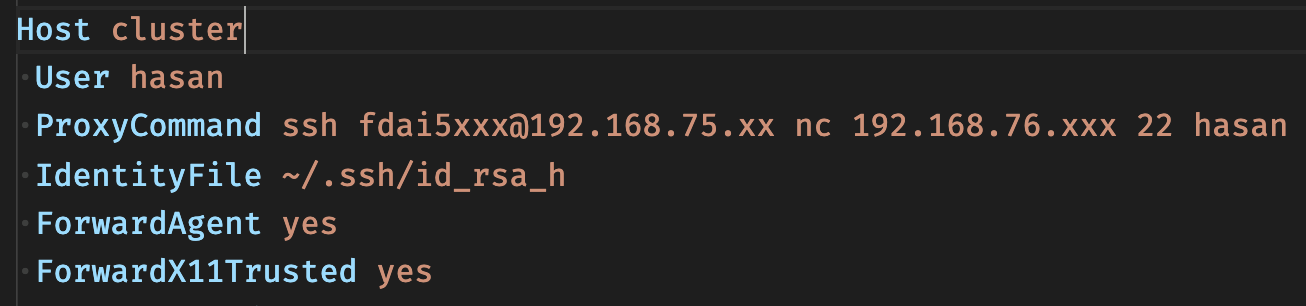
\includegraphics[scale=0.55]{images/Chapter4/ssh_connection.png}
      \caption{SSH connection to GPU-Heavy Cluster}
      \label{fig:ssh_connection}
    \end{figure}
  \end{itemize}

\subsection{Python}\label{subsec:python}
Python is a general purpose, platform independent and high level programming language. It is used for developing desktop GUI applications, web applications and machine learning. Python is the perfect choice for beginners to make your focus on in order to jump into the field of data science and machine learning. It is a stable, flexible, concise, readable and intuitive language with a wide community and full-featured libraries/frameworks which significantly reduces the time required to get your first results. While complex algorithms and versatile workflows stand behind machine learning and AI, the simplicity of Python makes it possible for developers to write robust programs.
% \subsection{Virtualenv}
% vir
\subsection{Tensorflow}
TensorFlow\cite{tensorflow} is basically an open-source Python programming library that contains common machine learning mathematical operations designed to simplify development and deployment of ML powered applications. The library helps users to communicate these mathematical operations as a data flow graph representing the movement of data between operations. The API also speeds up mathematically intensive neural networking and machine learning algorithms on multiple components of CPU and GPU, including optimal CUDA extensions for Nvidia GPU. Tensorflow is the result of Google's long term vision and research in machine learning.
\subsection{Keras}
Keras\cite{keras} is a high-level neural networks API, written in Python. It helps in building, training and testing machine learning models easily using its intuitive high-level APIs with eager execution, which makes for immediate model iteration and easy debugging. The main reasons for using Keras is its user-friendliness, fast learning and model building. You can rapidly prototype a simple or very complex neural networks within a few minutes using Keras. The Model and the Sequential APIs are so powerful that you can do almost everything you may want. Keras provides the benefits of wide adoption and support for a variety of application delivery solutions, compatibility with at minimum five back-end engines (TensorFlow, CNTK, Theano, MXNet, and PlaidML), and strong support for several GPUs and distributed training. Secondly, Keras is backed by Google, Microsoft, Apple, Amazon, Uber, Nvidia, and others. Keras follows the best practices for diminish cognitive load: it exposes a consistent and simple APIs, it reduces the number of user actions required for common use cases, and it provides clear and actionable feedback upon user error.
\subsection{NumPy}
NumPy\cite{numpy} is an open-source general-purpose array-processing Python library. NumPy comprises a multi-dimentional array and matrix data structures. It can be used to run a variety of mathematical operations on arrays such as trigonometric, algebraic and quantitative routines. We have used Numpy a lot to manipulate data. NumPy is an expansion of Numeric and Numarray and Pandas is built around the NumPy array.
\subsection{OpenCV}
OpenCV\cite{opencv} is a cross-platform library which is used to develop real-time computer vision applications and to boost the use of machine perception in the commercial products. OpenCV makes it easy for businesses to use and edit the code. We have used pretty basic features of OpenCV during this project like to load, resize and show images. Some of the things that OpenCV can do out of the box are as following:
\begin{itemize}
  \item Image processing operations.
  \item Video analysis.
  \item Building GUI.
  \item 3D reconstruction.
  \item Feature extraction.
  \item Object detection.
  \item Machine learning.
\end{itemize}
% opencb
% \par
% Before diving deep into the implementation of different solutions for document classification, let's go through some of the major tools and technologies which we used in different solutions.
% \subsection{Python}
% Python is one of the most popular and powerful open-source backend programming language. The main reason for its popularity is easy to use syntax. We can do wonders by writing very few lines of code. Also, python is one of the most used language in the domain of machine learning due to its enormous support and libraries for machine learning and deep learning such as Tensorflow, Scikit-learn, PyTorch, Numpy, Keras, etc.
% \subsection{Tensorflow}
% Tensorflow is an open-source machine learning library developed by Google and released as an open-source project in 2105 for implementing machine learning algorithms. It offers high-level APIs for the implementation of machine learning algorithms so that we don't have to go really deep for writing complex code to develop a neural network or to even configure or program a neuron. It also provides both C++ and Python APIs that makes it easier to work on and has relatively faster compilation time than other Deep Learning libraries. Tensorflow supports both CPU's and GPU's computing devices.
% \subsection{Keras}
% Keras is a deep learning TensorFlow library to implement deep neural networks very quickly. Why most of the developers are switching to kaggle because it is providing high-level APIs of TensorFlow implementation to implement and configure neural networks. You can use Kaggle Sequential or Functional API to build a neural network from scratch or either use transfer learning models provided as an API by Keras. It provides multiple functions to configure the neural network model like add, fit, compile, evaluate, predict, etc.
% \subsection{Scikit-learn}
% Scikit learn is another very powerful machine learning library used by the developers to implement machine learning algorithms. It contains many tools for supervised and unsupervised machine learning and statistical modeling. It is built on SciPy and primarily used for data modeling.
% \subsection{Kaggle}
% Kaggle is an online free platform for data scientists to create, implement and search machine learning and data science solutions. It provides several features like Datasets where you can search and use or even download the datasets which are published publicly. Most of the machine learning developers use kaggle to find the dataset for their machine learning problems. Along with that, it also provides a development environment in the form of Jupyter Notebook called Kaggle Kernels. This notebook can be used to run python or R programming language. The reason for its popularity is that it provides very high-level computing power specifically GPU computing and currently allowing to upload up to 10GB of data free.
% \subsection{Pytesseract}
% Python-tesseract is an optical character recognition (OCR) tool for python. It is primarily used for reading or extracting text from images. Python-tesseract is a wrapper for Google's Tesseract-OCR Engine.
% \section{Evaluation Metrics}
% In machine learning projects, after training the model for a problem, it is very necessary to check and evaluate its performance before using it in any live system. For this purpose, there are various metrics and techniques to measure performance. In this section, we will describe a few of the techniques for model's performance evaluation
% \subsection{Model Accuracy}
% Whenever we have to check how well our model has trained, our first step is to check the final average classification accuracy of the model which is shown in percentage indicating the confidence score and how well the model has learned from the training data. The formula for calculating accuracy is to divide the number of correct predictions during training out of the total number of predictions. When we compile the model after passing the data and setting parameters, it shows the accuracy along with the loss value for each epoch and after completing all the epochs it returns the average classification accuracy of the model.
% \subsection{Loss}
% Through loss value, we evaluate how well our training algorithm modeling the input dataset.  If the predictions are not as expected, then it gives a higher number. If the predictions are good and as expected, then the output will be a smaller number. This output in the form of a number and is called loss value which indicates whether our training model is well trained for the given dataset or not.  If the loss value is within the threshold then our model is fine and good to go but in case the loss value is very high, then there are some additional steps need to perform to minimize the loss value.  In the case of higher loss values, we optimize or tune our weights for the model. Here, weights are the numerical value which are the parameters set for our model.
% \subsection{Confusion Matrix}
% A confusion matrix is an evaluation metric to check the classification performance of a trained machine learning model. Normally, after training the model with training data, we use test data to check how well our model is working on the data which was not present during training. After that, we create a confusion matrix to check the performance which indicates the number of true predictions. Basically, it returns a matrix with n number of rows and columns where n is the number of classes for which the model is trained. Please see the Figure \ref{cm} to see a result of a confusion matrix.
% \begin{figure}[H]
% \centering
% 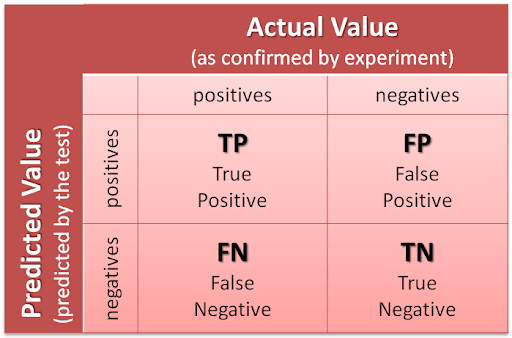
\includegraphics[scale=0.7]{images/Chapter5/cm.png}
% \caption{Illustration of a Confusion Matrix \cite{conf_matrix}}
% \label{cm}
% \end{figure}
% \par
\section{Implementation \& Evaluation for Solution I}
% As mentioned earlier, this solution is based on a custom algorithm which is accepting textual information and apply some scoring function to determine the type of the document. Let's discuss the solution in detail and evaluate the performance.
% \subsection{Proposed solution}
% This solution starts with creating the dictionary of relevant words. Although, we are using some metrics to generate the dictionary by extracting text from pdf but still it requires some manual filtration of garbage words. Later on, we use this dictionary to filter the garbage data while text extraction and analysis anywhere. After generating the dictionary, we extract the text from pdfs and then categorize the text by document types. Since, this solution is not using any machine learning techniques, so we are not using high amount of data to categorize the data. Please find below the Figure \ref{text_cat_data} to see the data after applying text categorization. 
% \begin{figure}[H]
% \centering
% 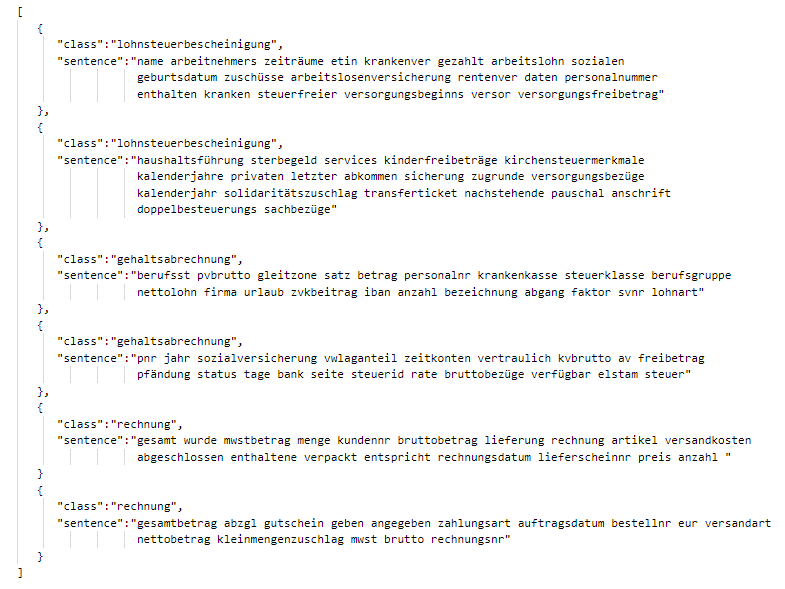
\includegraphics[scale=0.9]{images/Chapter5/sol_1/sol1-data.png}
% \caption{Text categorization data by Document Type}
% \label{text_cat_data}
% \end{figure}
% \par
% This categorization is further used to generate class words and corpus. As seen in the above figure  this list contains the sentences belongs to a particular document type but class words contains the list of words by each document type. Please see the Figure \ref{class_words} for the reference. On the other hand, the corpus is something which is independent of categorization and contain the list of words with its frequency of occurrences throughout the data or in other terms the commonality of each word. Please see the Figure \ref{corpus} for the reference.
% \begin{figure}[H]
%   \centering
%   \begin{minipage}[b]{0.4\textwidth}
%     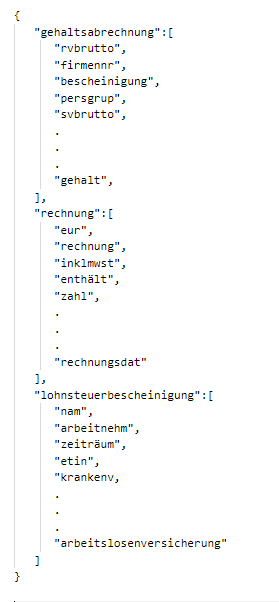
\includegraphics[scale=0.9]{images/Chapter5/sol_1/class_words.png}
%     \caption{Class words data by Document Type}
%     \label{class_words}
%   \end{minipage}
%   \hfill
%   \begin{minipage}[b]{0.4\textwidth}
%     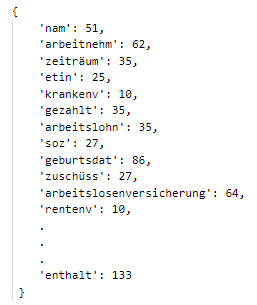
\includegraphics[scale=0.9]{images/Chapter5/sol_1/corpus_words.png}
%     \caption{Corpus reflecting words commonality}
%     \label{corpus}
%   \end{minipage}
% \end{figure}

% \par
% We are using class words and corpus in scoring function for the solution. Now, when we are done with lists of words with weight and by document types, we can do the classification. What is happening in text classification in this solution is that we extract the text from the document and pass it to our classification function which analyzes the textual information and calculates the score for each document type on the basis of this text and ultimately returns the class with the highest score. The classification function is using another method that is responsible for calculating the score for any document type. Please see Listing \ref{score_func} to see the implementation of calculating the class score. Here we are using a formula and corpus and class words for apply scoring and treat each word with relative weight.
% \begin{listing}
% % \inputminted[frame=lines,framesep=2mm,baselinestretch=1.2,fontsize=\scriptsize,linenos]{python}{Chapter5/classification_func.py}
% \caption{Function to calculate class score}
% \label{score_func}
% \end{listing}
% \subsection{Evaluation}
% For the evaluation of performance, we used another generated dataset. We applied the above methodology to classify the document type by calculating the word frequency score for each type and found out that it is working fine with full accuracy and zero error rate. Please find below the Figure \ref{sol1_eval} to see evaluation results.
% \begin{figure}[H]
% \centering
% 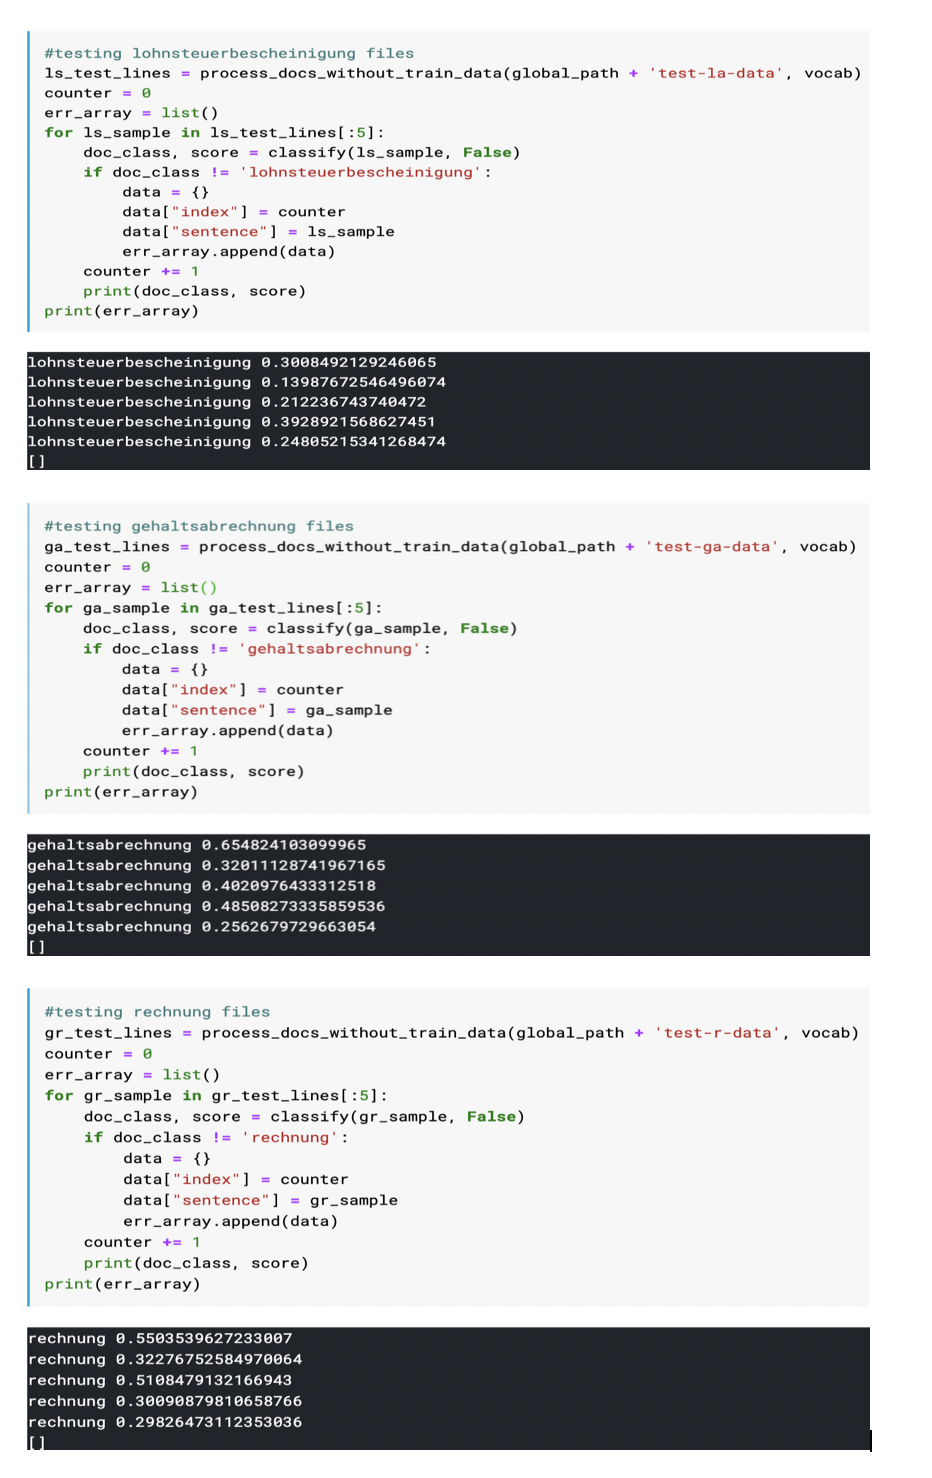
\includegraphics[scale=0.7]{images/Chapter5/sol_1/sol1_eval2.png}
% \caption{Evaluation of solution by Document Type}
% \label{sol1_eval}
% \end{figure}
% \section{Implementation \& Evaluation for Solution II}
% In this solution, we developed and trained a ConvNet by using Keras Sequential API. We are using textual content as the source of input to train the model. In the further sections, we will describe the neural network architecture proposed for training the model and its evaluation which is carried out on testing data.
% \subsection{Proposed Neural Network Architecture}
% The neural network developed for this solution is trained to predict the document types of tax-related documents. The network accepts the textual data in the form of vector input for training and is consists of 3 layers. The number of layers decided by considering the complexity of the problem in this solution. Please see Figure \ref{sol2_network_details} to know the details of the neural network used. Out of 3 layers, there are two core layers each consists of 50 nodes, where the first layer is using \q{ReLU} as an activation function, followed by a final output layer with nodes equal to the number of document types(classes) we are using. The output layer is using \q{Sigmoid} as an activation function for the prediction of the document type.
% \begin{figure}[H]
% \centering
% 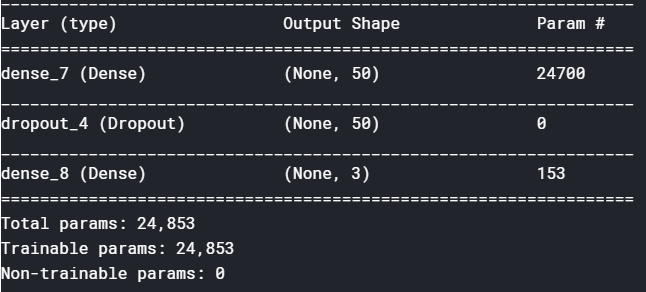
\includegraphics[scale=0.7]{images/Chapter5/sol_2/network_detail_sol2.png}
% \caption{Details of Neural Network used for Solution II}
% \label{sol2_network_details}
% \end{figure}
% \par
% The idea behind the implementation is to use the textual information extracted from the documents. Here, documents can be in the form of pdfs or images. After the text extraction, we apply some data processing steps where we filter the irrelevant and garbage words from the text. Furthermore, the text extracted from a single document is further broke down into small strings and applied word shuffling to introduce the distinguishing factor between the input text records. After applying all the above things, we have now a list of string where each string consists of multiple keywords related to a specific document type. Later on, we apply the bag of word approach to convert this raw text into an integer vector array so that it can be used to train the model. We used Keras Tokenizer API \cite{keras_tokenizer} to convert the text into a vector array. The Tokenizer API provides different modes to convert text to vectors. We tried different modes and found that \q{Frequency} mode works best for our problem. So, after applying the Tokenizer API, we have the vector array which we use to train our model.
% \subsection{Training the Model}
% At this stage, after processing our data, we are training our neural network model which is supposed to predict the document type of tax documents. Here, I would mention that we are using only three types of documents with limited formats because of the lack of data and this trained model will recognize only one document type at a time instead of giving confidence score for each document type. The parameters used to train the model are very few and needed a little bit tweaking by hit and trial to achieve the good results. Please see the below List \ref{hp_md_sol2} to know the data and parameters used to train the model.
% \begin{table}[H]
% \centering
% \begin{tabular}{l  l  l}
%  & Types/Parameters & Value \\
% \hline
% \\ Dataset & Lohnsteuerbescheinigung(Income Tax Statement) & 12800 \\
%       & Gehaltsabrechnung (Salary slips) & 7202 \\
%       & Rechnung (General Receipts) & 3653  \\\\
      
% \hline
% \\ Model & Layers & 3 \\
%     & Activation Function (Output layer) & Sigmoid \\
%     & Epochs & 30 \\
%     & Trained for number of classes & 3 \\\\
% \end{tabular}
% \caption{Parameters setting for model training}
% \label{hp_md_sol2}
% \end{table}
% \par
% In the above list, the dataset values reflect the number of records generated by extracted text from documents and break down the text into further small strings. Why the values are not equal for each document type is because the General receipts do not contain as much text as the income tax statement and salary slips.
% \subsection{Evaluation}
% In this step, after training the model, it's time to evaluate the performance that how well the model is trained and how well it has generalized the training data. To find out this, we first check the final accuracy of the model and the final loss. Furthermore, to evaluate the model further, we used the test data and checked the predictions on it.
% \subsubsection{Final Accuracy \& Loss}
% \begin{figure}[H]
% \centering
% 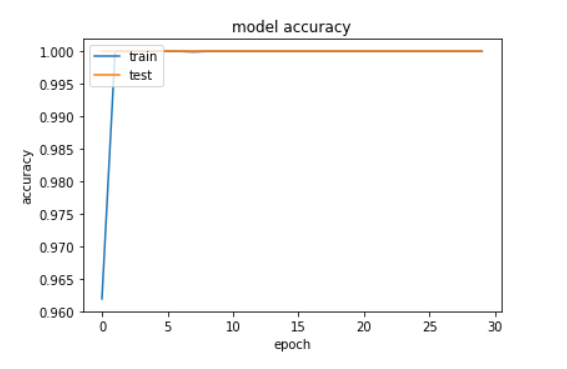
\includegraphics[scale=0.7]{images/Chapter5/sol_2/acc_graph.png}
% \caption{Final Accuracy of the trained model for Solution II}
% \label{acc_sol2}
% \end{figure}
% \par
% We trained our neural network with 30 epochs and got the final average accuracy of 100\%. If we see the Figure \ref{acc_sol2}, we will see that we are getting a high accuracy of around 96\% for training data from the very first epoch and after that, the accuracy remains constant of 100\% for the rest of epochs however for test data we are getting the 100\% accuracy since the beginning. Although this may indicate a scenario of overfitting but, it needs to understand the nature of data at this stage. In our data, each input record contains more or less same kind of data with a little bit of variation for each document type which makes this problem very simple to understand for the model.
% \begin{figure}[H]
% \centering
% 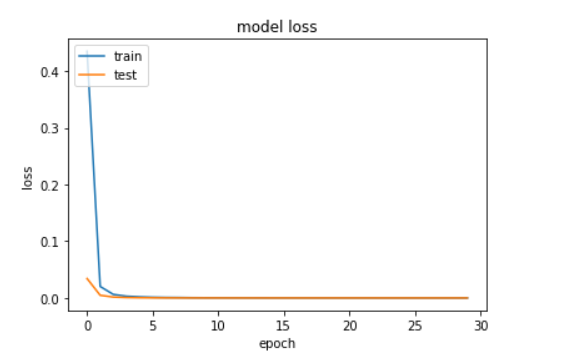
\includegraphics[scale=0.7]{images/Chapter5/sol_2/loss_graph.png}
% \caption{Final Loss of the trained model  for Solution II}
% \label{loss_sol2}
% \end{figure}
% \par
% Whereas, if we see the graph of loss value in Figure \ref{loss_sol2} for the model then again, we are getting a very low final loss value of 0.000404. The loss value needs to be as low as possible to have a well-trained model. For the training data, the loss value starts at 0.4 on the first epoch and then decreased to almost 0 after that whereas the test data started with the low loss value from the beginning.
% \subsubsection{Confusion Matrix}
% \begin{figure}[H]
% \centering
% 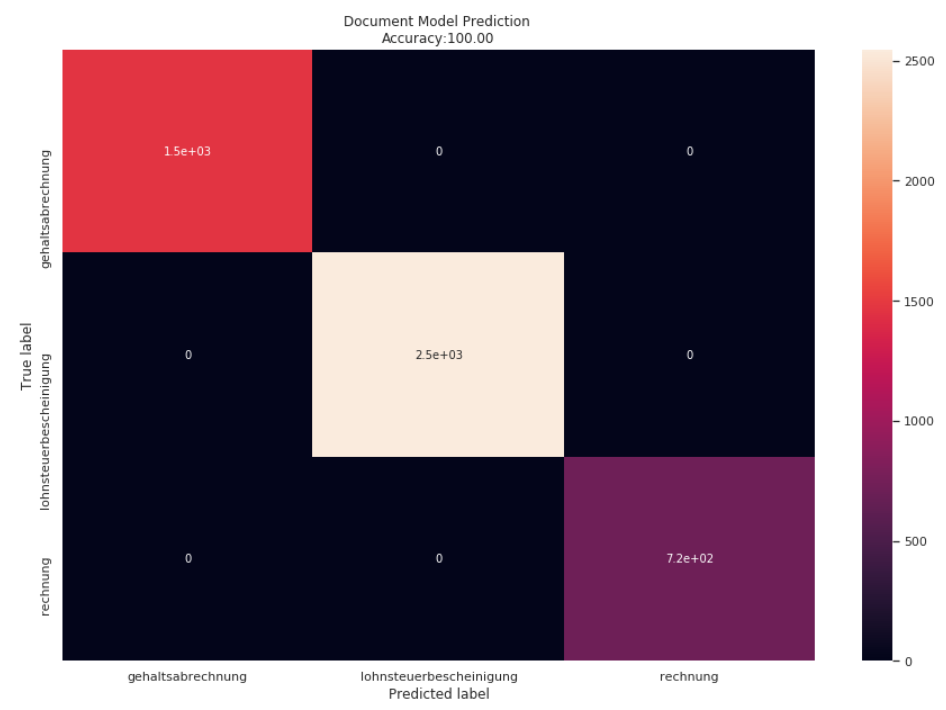
\includegraphics[scale=0.7]{images/Chapter5/sol_2/cm-sol1.png}
% \caption{Confusion Matrix for 3 Document types  for Solution II}
% \label{cm_sol2}
% \end{figure}
% \par
% After training the model, we evaluated our model by making predictions on the test data which is not present during the training and is totally new for the model. Here, the model again achieved the accuracy of 100\% by placing the correct labels to each prediction. To find out the accuracy, we can refer to the Figure \ref{cm_sol2} which reflects the confusion matrix of the model for the predictions on testing data. Here, we used a total of 4731 records for the testing and as you can see the matrix all the records predicted correctly.
% \subsubsection{Classification Report}
% \begin{figure}[H]
% \centering
% 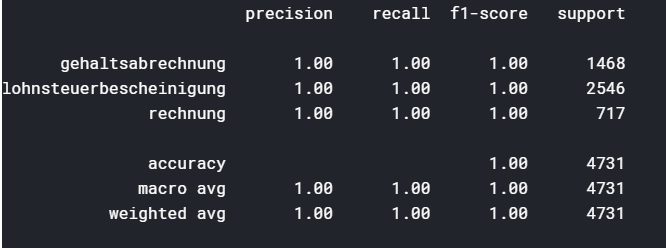
\includegraphics[scale=0.9]{images/Chapter5/sol_2/classification_report.png}
% \caption{Classification Report for 3 Document types  for Solution II}
% \label{cr_sol2}
% \end{figure}
% \par
% The classification report also verifies the results of the confusion matrix that all the document types achieved the f1-score of 100. Also, the weighted average and accuracy of all of them showing the good numbers.
% \section{Implementation \& Evaluation for Solution III}
% In the third solution which is our main solution, unlike the previous solution, we are leveraging the service of transfer learning using Keras to develop and train our ConvNet model instead of creating the model from scratch. Also, the form of input is changed, as in this solution we are not relying on the textual content inside the document but instead we are giving visual information of document for the training of model by converting the pdfs into images. In further sections, we will describe the network proposed for this solution along with the different experiments carried out and its evaluation.
% \subsection{Proposed Neural Network Architecture}
% \begin{figure}[H]
% \centering
% 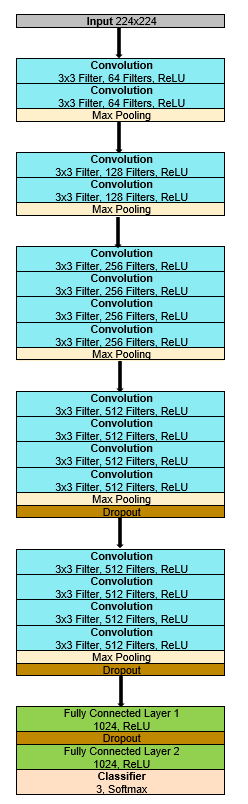
\includegraphics[scale=0.9]{images/Chapter5/sol_3/sol3_arch.png}
% \caption{Network Architecture used for Solution III }
% \label{network_arch_sol3}
% \end{figure}
% \par
% The neural network used in this solution is totally different from the network used in Solution II. Here, we used the above VGG19 architecture to develop the neural network which was again designed to predict the tax-related documents. This network accepts visual data in the form of images exactly of size 224x224 pixel as per the requirement of the VGG19 model for training. The network consists of a total of 19 layers and contains convolutional layers of filter size 3x3 and using ReLU for activation function. On top of the network, two fully connected layers of 1024 nodes using ReLU as an activation function is attached. In the end, there is an output layer that uses Softmax for activation function and has nodes equal to the number of classes which in our case is 3 and is responsible for predicting the document types.
% \newline
% \par
% Before passing the data to the model for training, we applied some pre-processing to image dataset in the form of image augmentation. Various parameters are used to transform the images into different shapes. In our case, it was very important and helpful because of the nature of data and also due to the lack of data. The transformation involves rotation of images, zooming in, horizontal and vertical flips, height and width shift, etc. Please see Figure \ref{aug_data} in Chapter \ref{chap:3} to see the effects after augmentation.
% \subsection{Training the Model}
% After the pre-processing of images, our dataset is ready for the model training. Again, the purpose of this model is the same as the previous model in Solution II that is we are training this model to determine one tax document type at a time unlike the multi-label classification and the classes are also the same. For training the model, we carried out different experiments by changing the hyperparameters and augmentation parameters of the model to see the results. In the below List \ref{hp_mdl_1}, you can find out the data and parameters used to train the model.
% \begin{table}[H]
% \centering
% \begin{tabular}{l  l  l}
%  & Types/Hyperparameter & Value \\
% \hline
% \\ Dataset & Lohnsteuerbescheinigung(Income Tax Statement) & 4000 \\
%       & Gehaltsabrechnung (Salary slips) & 4000 \\
%       & Rechnung (General Receipts) & 4200  \\\\
% \hline
% \\ Model & Input Size & 224x224 \\
%       & Batch Size & 64 \\
%       & Optimizer & SGD \\
%       & Learning Rate & 0.001 \\
%       & Momentum & 0.9 \\
%       & Epochs & 50 \\\\
% \hline
% \\ Regularization & Early Stopping & Yes \\ \\
% \hline
% \\ Preprocessing & Centering & Yes \\ 
%                  & Re-size   & Yes, 224x224 \\ \\
% \hline
% \\ Augmentation & Rotation Range & \ang{10}  \\ 
%                 & Re-scale Image & multiply pixels by 1/255.0 \\ 
%                 & Width Shift Range & 0.1 \\ 
%                 & Height Shift Range & 0.1 \\ 
%                 & Zoom Range & 0.2 \\ 
%                 & Horizontal Flip & Yes \\ 
%                 & Vertical Flip & No \\ 
%                 & Brightness Range & No \\ \\
% \hline
% \end{tabular}
% \caption{Dataset and Hyperparameters for the model}
% \label{hp_mdl_1}
% \end{table}
% \par
% In this model training, we are using the image dataset in the above-mentioned quantity for each document type. As mentioned, we used the VGG19 model for our model, so we used Keras to create our model and initialized it with the ImageNet database. The reason to initialize the model with ImageNet is that ImageNet contains the generic data of more than 1000 categories so by using ImageNet we can leverage the training of core layers already trained on the ImageNet dataset. On top of that, we applied our newly added two fully connected layers and output layer for the final prediction of the documents.
% \subsection{Evaluation}
% Once the model is trained, now we can evaluate the performance of the trained model. In this solution, we have used the same evaluation metrics that we used in Solution II. After the training, we checked the final accuracy and loss of the model which we will see in the next section. Along with that, we checked the predictions on test data and based on that we generated the confusion matrix and classification report for our model generalization.
% \subsubsection{Final Accuracy \& Loss}
% \begin{figure}[H]
% \centering
% 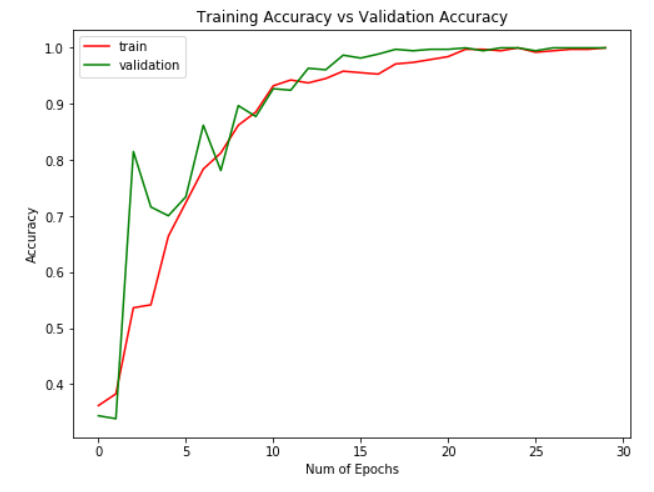
\includegraphics[scale=0.8]{images/Chapter5/sol_3/ac3_sol3.png}
% \caption{Final Accuracy of the trained model for Solution III }
% \label{acc_sol3}
% \end{figure}
% \par
% We trained our neural network model with 50 epoch and achieved the final average classification accuracy of 100\%. If we compare the accuracy of this solution to Solution II, we can clearly see from Figure \ref{acc_sol3} that the accuracy is increasing gradually till the final epochs, unlike Solution II where we achieved the accuracy of 100\% right after the first epoch. Here, on training data, the accuracy started with 32 percent with the first epoch and saw the increase of 5-10 percent on average in each epoch while on validation data, the accuracy starts a little bit lower than the training data but in the end, it achieves the same accuracy as of on training data. Overall the graph is indicating very good results.
% \begin{figure}[H]
% \centering
% 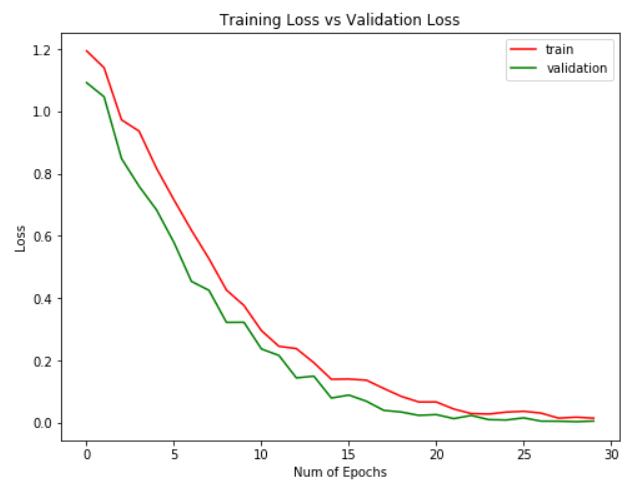
\includegraphics[scale=0.8]{images/Chapter5/sol_3/loss3_sol3.png}
% \caption{Final Loss of the trained model for Solution III}
% \label{loss_sol3}
% \end{figure}
% \par
% If we talk about the training and validation loss, in Figure \ref{loss_sol3} the graph is pretty good and reflects the gradual decrease in the loss values of our model. On training data, the loss value started around 1.2 on the first epoch and then decreases gradually and by the final epoch, the loss value was around 0.02. Also, it should be noted that there is no crunch in the loss value means the loss value didn't increase throughout the training. On the validation data, the loss value started at 1.1 and in the end, matches the values of training loss.
% \subsubsection{Confusion Matrix}
% \begin{figure}[H]
% \centering
% 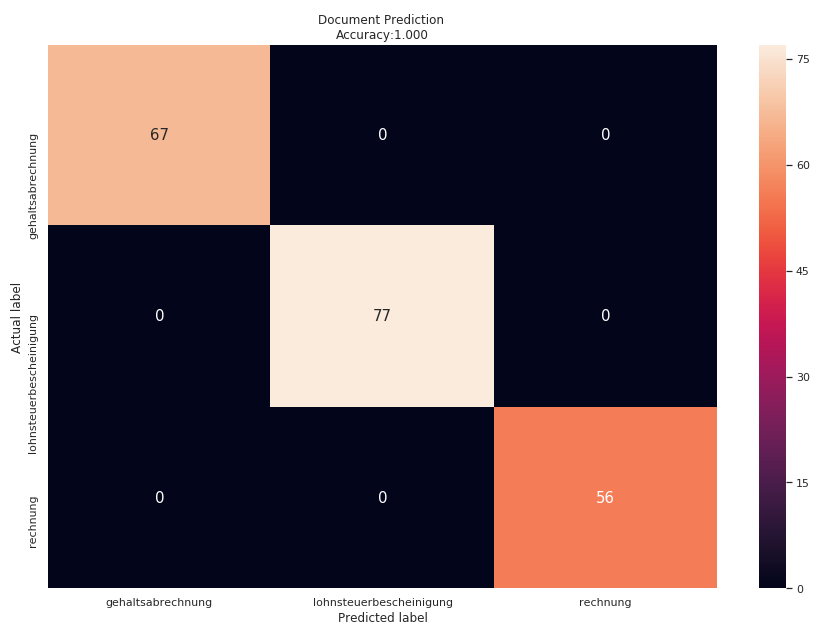
\includegraphics[scale=0.8]{images/Chapter5/sol_3/cm3_sol3.png}
% \caption{Confusion Matrix for 3 Document types for Solution III }
% \label{cm_sol3}
% \end{figure}
% \par
% We also evaluated the performance of our model by checking how well the model is predicting on testing data which were not used during the training and found out that the model is predicting accurately for each class of our document types by creating a confusion matrix and achieves an accuracy of 100\% on average. This indicates the generalization of our model. For the testing, we used a total of 200 images for all types of documents. Please see Figure \ref{pred_sol3} for seeing the prediction results of our model on the testing data.
% \begin{figure}[H]
% \centering
% 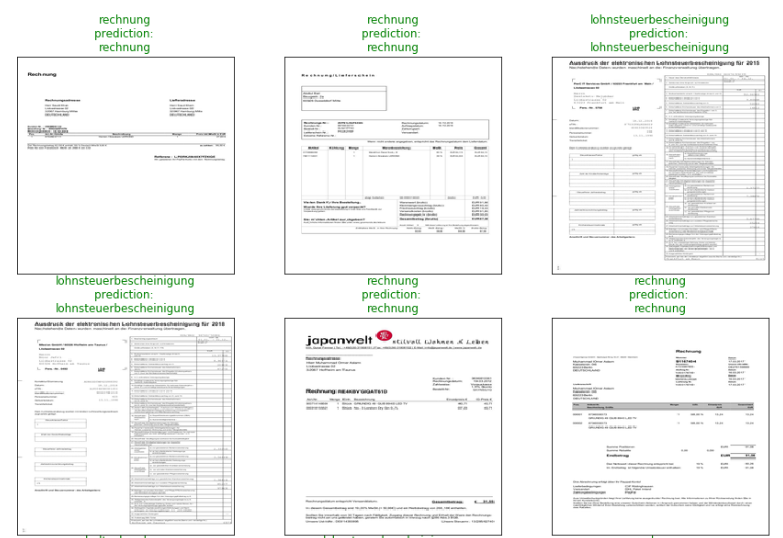
\includegraphics[scale=0.9]{images/Chapter5/sol_3/predictions_sol3.PNG}
% \caption{Model Predictions of labels on testing data }
% \label{pred_sol3}
% \end{figure}
% \subsubsection{Classification Report}
% \begin{figure}[H]
% \centering
% 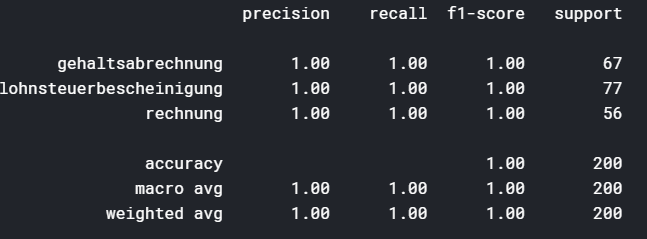
\includegraphics[scale=0.8]{images/Chapter5/sol_3/cr3_sol3.png}
% \caption{Classification Report for 3 Document types for Solution III }
% \label{cr_sol3}
% \end{figure}
% \par
% From the classification report, it also verifies the results of the confusion matrix that all the document types achieved the f1-score of 100. Also, the weighted average and accuracy of all of them showing the good numbers.